\section{Improving Deep Neural Networks: Hyperparameter tuning, Regularization and Optimization}
This is the second courseof deep learning specialization at Coursera taught by Professor Andrew Ng. Here is my certificate after finishing this course (Fig. \ref{course2-cert}):

\begin{figure}[!htbp]
    \centering
    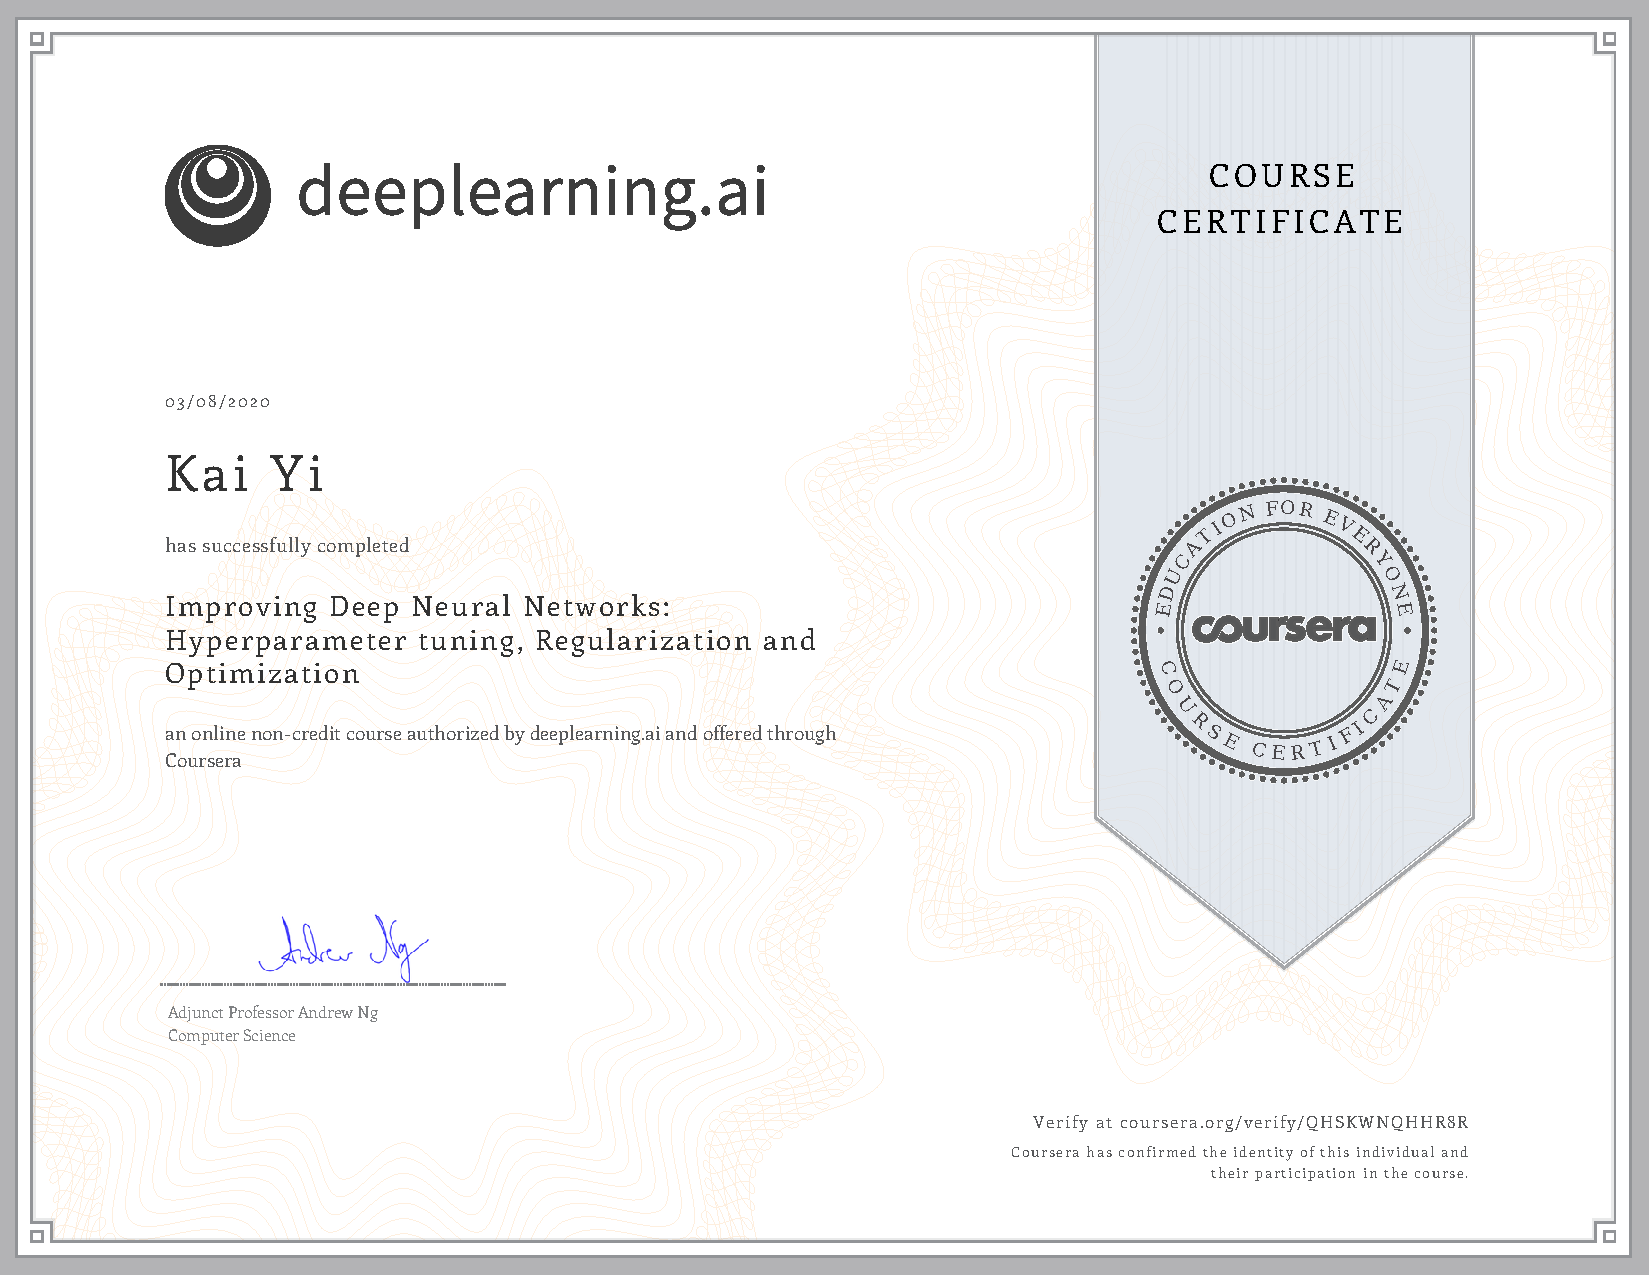
\includegraphics[width=1.0\textwidth]{img/C2-Certificate.pdf}
    \caption{Certificate of Improving Deep Neural Networks: Hyperparameter tuning, Regularization and Optimization. Obtained in March 2020.}
    \label{course2-cert}
\end{figure}

\subsection{Course Overview}
According to the official site of this course, there are following key components:

\begin{itemize}
    \item Understand industry best-practices for building deep learning applications.
    \item Be able to effectively use the common neural network 'tricks', including initialization, L2 and dropout regularization, batch normalization and gradient checking.
    \item Be able to implement and apply a variety of optimization algorithms, such as mini-batch gradient descent, momentum, RMSprop and Adam, and check for their convergence.
    \item Understand new best-practices for the deep learning era of how to set up train/dev/test sets and analyze bias/variance.
    \item Be able to implement a neural network in TensorFlow.
\end{itemize}

\subsection{Practical Aspects of Deep Learning}
\subsubsection{Train/Dev/Test Sets}
Pipeline of deep learning practice: Idea $>>$ Code $>>$ Experiment $>>$ Idea. We get initial idea first, then implement the rough idea. Next fine tuning our model based on experiment. Then we get new thoughts.

Data will be split into three parts:

\begin{itemize}
    \item Training Set. (the largest set)
    \item Hold-Out Cross Validation Set / Development Set.
    \item Test Set.
\end{itemize}

We will try to build a model upon training set then try to optimize hyperparameters on dev set as much as possible. Then after our model is ready we try and evaluate the testing set.

Thus the trend on the ratio of splitting the models:
\begin{itemize}
    \item If size of the dataset is 100 to 1,000,000, then $=>$ 60/20/20.
    \item If size of the dataset is more than 1,000,000, then $=>$ 98/1/1 or 99.5/0.25/0.25.
\end{itemize}

Make sure the dev and test set are coming from the same distribution. 

\begin{itemize}
    \item E.g. The cat training pictures from the web can be put into training set to get more data. However, the picture from users cell phone and the web have different distribution. Therefore, the web picture can not be used separately on dev set or test set. Besides, it's better not to use a little web picture on dev/test set (it will cause mismatch problem). Besides, 
\end{itemize}

It's OK to only have a dev set without a testing set. But a lot of people in this case call the dev set as the test set. A better terminology is to call it a dev set as its used in the development.

\subsubsection{Bias / Variance}
Bias / Variance techniques are easy to learning, but difficult to master.

\begin{itemize}
    \item Underfitting $=>$ High Bias
    \item Overfitting $=>$ High Variance
\end{itemize}

The following visualization (Fig. \ref{bias-variance}):

\begin{figure}
    \centering
    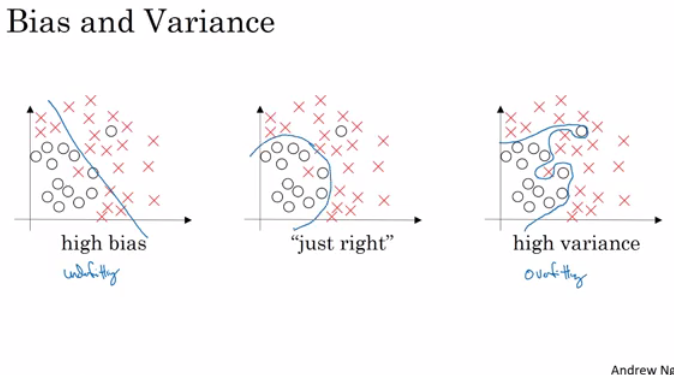
\includegraphics[width=1.0\textwidth, trim={0 70, 0 60}, clip]{img/c2/bias-variance.png}
    \caption{Bias and Variance.}
    \label{bias-variance}
\end{figure}

If Bayesian error (optimal error) is 0\%, next is several cases:

\begin{itemize}
    \item High variance (overfitting): Train error: 1\%, Dev error: 15\%
    \item High bias (underfitting): Train error: 10\%, Dev error: 8\%
    \item High bias \& high variance: Train error: 16\%, Dev error: 30\%
    \item Quite well: Train error: 0.6\%, Dev error: 0.9\%
\end{itemize}

\subsubsection{Basic Recipe for Machine Learning}
If my algorithm has a high bias:
\begin{itemize}
    \item Try to make my NN bigger (size of hidden units, number of layers).
    \item Try to train it longer.
    \item (Not unique) Try a different model that is suitable for my data / Try different (advanced) optimization algorithms.
\end{itemize}

If my algorithm has a high variance:
\begin{itemize}
    \item Get more data.
    \item Try regularization.
    \item (Not unique) Try a different model that is suitable for my data / Try different (advanced) optimization algorithms.
\end{itemize}

I should try the previous two points until I have a low bias and low variance.

In the older days before deep learning, there was a 'Bias/Variance Tradeoff'. But nowadays we can reduce bias and variance separately by using more advanced tools and techniques.

\subsubsection{Regularization}
Adding regularization to NN will help it reduce variance (overfitting).

\begin{itemize}
    \item L1 matrix norm: $||W|| = \sum w_{ij}$.

    \item L2 matrix norm: $||W||^2 = \sum w_{ij}^2$. Also $||W||^2 = W^T * W $ if W is a vector.
\end{itemize}

Regularization for logistic regression: (Find more accurate equations for regularizations)
\begin{itemize}
    \item The normal cost function that we want to minimize is: $J(W, b) = \frac{1}{m} \sum L(y_i, \hat{y}_i)$
    \item The L2 regularization version: $J(W,b) = \frac{1}{m} \sum L(y_i, \hat{y}_i) + \frac{\lambda}{2m} \sum w_i^2$
    \item The L1 regularization version: $J(W,b) = \frac{1}{m} \sum L(y_i, \hat{y}_i + \frac{\lambda}{m} \sum w_i$
    \item L2 regularization is being used much more often and $\lambda$ here is the regularization parameter (hyperparameter)
\end{itemize}

(Some points I can not understand very clearly here.)
% https://github.com/mbadry1/DeepLearning.ai-Summary/tree/master/2-%20Improving%20Deep%20Neural%20Networks

\subsubsection{Why regularization reduces overfitting?}
Here are som intuitions:

Intuition 1:
\begin{itemize}
    \item If $\lambda$ is too large - a lot of w's will be close to zeros which will make the NN simpler (I can think of it as it would behave closer to logistic regression).
    \item If $\lambda$ is good enough it will just reduce some weights that makes the neural network overfit.
\end{itemize}

Intuition2 (with tanh activation function):
\begin{itemize}
    \item If $\lambda$ is too large, w's will be small (close to zero) - will use the linear part of the tanh activation function, so we will go from non linear activation to roughly linear which would make the NN a roughly linear classifier.
    \item If $\lambda$ is good enought, it will just make some of tanh activations roughly linear which will prevent overfitting.
\end{itemize}

Implementation tip: if you implement gradient descent, one of the steps to debug gradient descent is to plot the cost function J as a function of the number of iterations of gradient descent and you want to see that the cost function J decreases monotonically after every elevation of gradient descent with regularization. If you plot the old definition of J (no regularization) then you might not see it decrease monotonically.

\subsubsection{Dropout Regularization}
The dropout regularization eliminates some neurons/weights on each iteration based on a probability. A most common technique to implement dropout is called "inverted dropout".

Code for inverted dropout:

\begin{lstlisting}[language=python]
keep_prob = 0.8 # 0 <= keep_prob <= 1, this code is only for layer 3

# the generated number that are greater than keep_prob will be 
# dropped. Thus 80% stay, 20% dropped.
# a3.shape = (num_neurons l3, m examples)
d3 = np.random.rand(a3.shape[0], a[l].shape[1]) < keep_prob

a3 = np.multiply(a3, d3) # only keep the values in d3 (True)

a3 = a3 / keep_prob # re-scaling a3, inverted dropout.
\end{lstlisting}

Matrix d3 is used for forward and back propagation and is the same for them, but it is different for each iteration due to the random initialization.

At test time we don't use dropout. If I implement dropout at test time - it would add noise to predictions.

\subsubsection{Understanding Dropout}
Intuition 1:
\begin{itemize}
    \item The intuition was that dropout randomly knocks out units in my network. So it's as if on every iteration I'm working with a smaller NN, and so using a smaller NN seems like it should have a regularizing effect.
\end{itemize}

Intuition 2:
\begin{itemize}
    \item NN can't rely on any one feature, so it has to spread out weights.
\end{itemize}

Dropout can have different keep\_prob per layer. And the input layer dropout has to be near 1 because I don't want to eliminate a lot of features.

A lot of researchers are using dropout in the area of computer vision because they have a very big input size and almost never have enough data, so overfitting is the usual problem. And dropout is a regularization technique to prevent overfitting.

A downside of dropout is that the cost function J is not well defined and it will be hard to debug (plot J by iteration).
\begin{itemize}
    \item To solve that I'll need to turn off dropout, set all the keep\_prob s to 1, and then run the code and check that it monotonically decreases J and then turn on the dropouts again.
\end{itemize}

\subsubsection{Other regularization methods}
\paragraph{Data Augmentation}
For example in a computer vision task:

\begin{itemize}
    \item Flip all my pictures horizontally which will give my more data instances
    \item Apply a random position and rotation to an image to get more data.
\end{itemize}

New data obtained using this technique isn't as good as the real independent data, but still can be used as a regularization technique.

\paragraph{Early Stopping}
In this technique we plot the training set and the dev set cost together for each iteration. At some iteration the dev set cost will top decreasing and will start increasing. 

We will pick the point at which the training set error and dev set error are best (great trade-off between dev error and train error). Thus we can take these parameters as the best parameters (Visualized at Fig. \ref{early-stopping}).

\begin{figure}[!htbp]
    \centering
    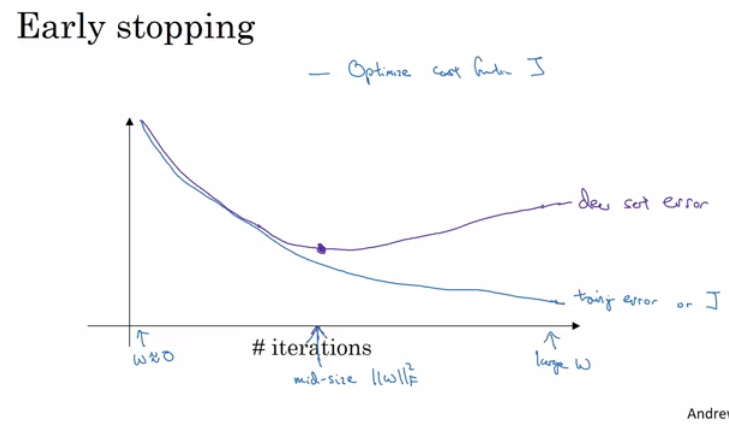
\includegraphics[width=1.0\textwidth, trim={30 30, 0 90}, clip]{img/c2/early-stopping.png}
    \caption{Early stopping method preventing overfitting.}
    \label{early-stopping}
\end{figure}

Professor Andrew prefers to use L2 regularization instead of early stopping because this technique simultaneously tries to minimize the cost function and not to overfit which contradicts the orthogonalization approach (we should not make decision on two variables).

However, the advantage of early stopping is that we don't need to search a hyperparameter like in other regularization approaches (like $\lambda$ in L2 regularization).

\paragraph{Model Ensembles}
Basic idea: Train multiple independent models and at test time average their results.

It can get 2\% improved performance and can be used in competitions instead of practical deployments. It reduces the generalization error. 

\subsubsection{Normalizing Inputs}
If I normalize my inputs this will speed up the training process a lot (convert optimizing from ellipse to circular).

Normalization are going on these steps:

\begin{itemize}
    \item Get the mean of the training set: mean = (1/m) * sum(x(i))
    \item Subtract the mean from each input: X = X - mean. This makes my inputs centered around 0.
    \item Get the variance of the training set: variance = (1/m) * sum((x(i)-mean)**2)
    \item Normalize the variance: X /= variance
\end{itemize}

These steps should be applied to training, dev, and testing sets (but using mean and variance of the train set).

Why normalize?
\begin{itemize}
    \item If we don't normalize the inputs our cost function will be deep and its shape will be inconsistent (elongated) then optimizing it will take a long time.
    \item But if we normalize it the opposite will occur. The shape of the cost function will be consistent (look more symmetric like circle in 2D example) and we can use a larger learning rate $\alpha$ - the optimization will be faster.
\end{itemize}


\subsubsection{Vanishing / Exploding gradients}
The vanishing / exploding gradients occurs when our derivatives become very small or very big.

To understand the problem, suppose that we have a deep neural network with number of layer L, and all the activation functions are linear and each b=0.

Then $\hat{Y} = W[L]W[L-1]\cdot W[1]X$. If we have 2 hidden units per layer and x1=x2=1, if W[i,j] is greater than 1, then $\hat{Y}$ will be exponentially large. Meanwhile, if W[i,j] is smaller than 1, then $\hat{Y}$ will be exponentially small.

\subsubsection{Weight Initialization for Deep Networks}
A partial solutions to the vanishing / exploding gradients in NN is better or more careful choice of the random initialization of weights.

A well chosen initialization can:

\begin{itemize}
    \item Speed up the convergence of gradient descent
    \item Increase the odds of gradient descent converging to a lower training (and generalization) error.
\end{itemize}

\begin{itemize}
    \item Zero Initialization: \textit{np.zeros(shape)}
    \item Random Initialization: \textit{np.random.randn(shape} * 0.01
    \item Bengio et al. Initialization: \textit{np.random.randn(shape) * np.sqrt(2/(n[l-1] + n[l])}
    \item He et al. Initialization (Xavier Initialization): \textit{np.random.randn(shape) + np.sqrt(2/n[l-1])} (Set ReLu as activation is better)
\end{itemize}

\subsubsection{Numerical approximation of gradients}
There is a technique called gradient checking which tells you if your implementation of backpropagation is correct.

There is a numerical way to calculate the derivative (Fig. \ref{gradient-checking})

\begin{figure}
    \centering
    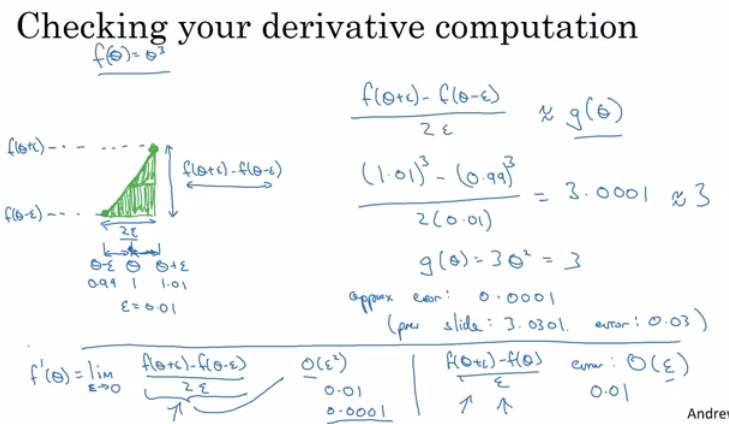
\includegraphics[width=1.0\textwidth, trim={0 0 0 35}, clip]{img/c2/gradient-checking.png}
    \caption{Checking the derivative computation.}
    \label{gradient-checking}
\end{figure}

Gradient checking is used only for debugging.

Main goal is to check whether the following satisfied:

\begin{equation}
    \frac{\partial J}{\partial \theta} = lim_{\epsilon \to 0}\frac{J(\theta + \epsilon) - J(\theta - \epsilon}{2\epsilon}
\end{equation}


% \begin{lstlisting}[language=python]
% epsilon = 1e-7
% for i in len(theta):
%     d_theta_approx[]
% \end{lstlisting}

% Adding more contents

\subsubsection{Gradient checking implementation notes}
Don't use the gradient checking algorithm at training time because it's very slow. Use gradient checking only for debugging. If algorithm fails grad check, look at components to try to identify the bug.

Don't forget to add $\frac{\lambda}{2m} \sum w_i$ to J if we're using L1 or L2 regularization.

Gradient checking doesn't work with dropout because J is not consistent. We must first turn off dropout, run gradient checking and then turn on dropout again.

Run gradient checking at random initialization and train the network for a while maybe there's a bug which can be seen when w's and b's become larger (further from 0) and can't be seen on the first iteration (when w's and b's are very small).

\subsubsection{Initialization Summary}
The weights should be initialized randomly to break symmetry.

It's OK to initialize the biases to zeros. Symmetry still can be broken so long as weights are initialized randomly.

Different initializations lead to different results.

Random initialization is used to break symmetry and make sure different hidden units can learn different things.

Don't initialize to values that are to large.

He initialization (Xavier Initialization) works well for networks with ReLU activations.

\subsubsection{Regularization Summary}
\paragraph{L2 Regularization}
The value of $\lambda$ is a hyperparameter that you can tune using a dev set. L2 regularization makes the decision boundary smoother. If $\lambda$ is too large, it's also possible to `oversmooth', resulting in a model with high bias.

\subparagraph{What is L2-regularization actually doing?} L2 regularization relies on the assumption that a model with large weights is simpler than one with small weights. Thus, by penalizing the square value of the weights in the cost function, you drive all the weights to smaller values. It becomes too costly for the cost to have large weights. This leads to a smoother model in which the output changes more slowly as the input changes.

\paragraph{Dropout}
Dropout is a regularization technique. You only use dropout during training. Don't use it (randomly eliminates nodes) during test time.

Apply dropout both during forward and backward propagation.

During training time, divide each dropout layer by keep\_prob to keep the same expected value for the activations. For example, if keep\_prob is 0.5, then we will on average shut down half the nodes, so the output will be scaled by 0.5 since only the remaining half are contributing to the solution. Dividing by 0.5 is equivalent to multiplying by 2. Hence, the output now has the same expected value. You can check that this works even when keep\_prob is other values than 0.5.

\newpage

\subsection{Optimization Algorithms}
% Continue to summarizing optimization algorithms.
% https://github.com/mbadry1/DeepLearning.ai-Summary/tree/master/2-%20Improving%20Deep%20Neural%20Networks#why-regularization-reduces-overfitting

\subsubsection{Mini-Batch Gradient Descent}
Training NN with large data is slow. So to find an optimization algorithm that runs faster is a good idea.

Suppose we have m = 50 million. To train this data it will take a huge processing time for one step. Because 50 million won't fit in the memory at once we need other processing to make such a thing.

In Batch Gradient Descent we run the gradient descent on the whole dataset while in Mini-Batch Gradient Descent we run the gradient descent on the mini datasets.

\begin{lstlisting}[language=python]
for t = 1:No_of_batches  # for every epoch
	AL, caches = forward_prop(X{t}, Y{t})
	cost = compute_cost(AL, Y{t})
	grads = backward_prop(AL, caches)
	update_parameters(grads)
\end{lstlisting}

The code inside an epoch should be vectorized. Mini-batch gradient descent works much faster in the large datasets.

\subsubsection{Understanding mini-batch gradient descent}
In mini-batch algorithm, the cost won't go down with each step as it does in batch algorithm. It could contain some ups and downs but generally it has to go down (unlike the batch gradient descent where cost function decreases on each iterations (Fig. \ref{mini-batch-gradient}).

\begin{figure}
    \centering
    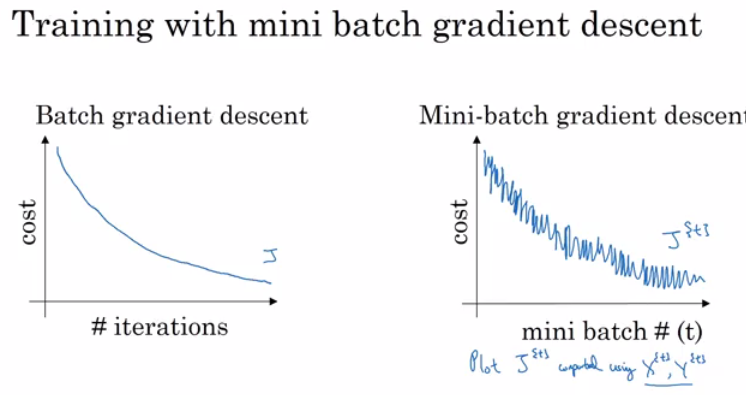
\includegraphics[width=1.0\textwidth, trim={0 35 0 70}, clip]{img/c2/batch_vs_mini_batch_cost.png}
    \caption{Training with mini batch gradient descent}
    \label{mini-batch-gradient}
\end{figure}

Mini-batch size:
\begin{itemize}
    \item (mini\_batch\_size = m) => batch gradient descent
    \item (mini\_batch\_size = 1) => stochastic gradient descent (SGD)
    \item (mini\_batch\_size =  between 1 and m) => ordinary mini-batch gradient descent
\end{itemize}

Batch gradient descent:
\begin{itemize}
    \item too long per iteration (epoch)
\end{itemize}

Stochastic gradient descent:
\begin{itemize}
    \item too noisy regarding cost minimization (can be reduced by using smaller learning rate)
    \item won't ever converge (reach the minimum cost)
    \item lose speedup from vectorization
\end{itemize}

Mini-batch gradient descent:
\begin{itemize}
    \item faster learning (you have the vectorization advantage and make progress without waiting to process the entire training set)
    \item doesn't always exactly converge (oscelates in a very small region, but you can reduce learning rate)
\end{itemize}

Guidelines for choosing mini-batch size:
\begin{itemize}
    \item If small training set (<2000 examples) - use batch gradient descent.
    \item It has to be a power of 2 (because of the way computer memory is layed out and accessed, somtimes your code runs faster if your mini-batch size is a power of 2): 64, 128, 256, 512, 1024, ...
    \item Make sure that mini-batch fits in CPU/GPU memory.
\end{itemize}

Mini-batch size is a hyperparameter.

\subsubsection{Exponentially weighted averages}
% Continue from \hyperref[here.]{https://github.com/mbadry1/DeepLearning.ai-Summary/tree/master/2-%20Improving%20Deep%20Neural%20Networks#exponentially-weighted-averages}.
There are optimization algorithms that are better than gradient descent, but you should first learn about Exponentially Weighted Averages.

If we have data like the temperature of day through the year it could be like this:

\begin{equation}
\begin{aligned}
\theta (1) & = 40\ \  (t(1) = 40)\\
\theta (2) &= 49\\
\theta (3) &= 45\\
&...\\
\theta (180) &= 60\\
&...
\end{aligned}
\end{equation}


This data is small in winter and big in summer. If we plot this data we will find it some noisy. 

Now lets computer the exponentially weighted averages:

\begin{equation}
    \begin{aligned}
    v0 &= 0\\
    v1 &= 0.9 * v0 + 0.1 * \theta(1) = 4\\
    v2 &= 0.9 * v1 + 0.1 * \theta(2) = 8.5\\
    v3 &= 0.9 * v2 + 0.1 * \theta(3) = 12.15\\
    &...
    \end{aligned}
\end{equation}

General equation:

\begin{equation}\label{ewa}
    v(t) = \beta v(t-1) + (1 - \beta) \theta (t)
\end{equation}

If we plot Equation \ref{ewa} it will represent averages over $ ~ \frac{1}{1-\beta}$ entries:

\begin{itemize}
    \item $\beta = 0.9$ will average last 10 entries
    \item $\beta = 0.98$ will average last 50 entries
    \item $\beta = 0.5$ will average last 2 entries
\end{itemize}

Best $\beta$ average for our case is between 0.9 and 0.98.

\paragraph{Intuition:} The reason why exponentially weighted averages are useful for further optimizing gradient descent algorithms is that it can give different weights to recent data points ($\theta$) based on value of $\beta$. If $\beta$ is high (around 0.9), it smoothens out the averages of skewed data points (oscillations w.r.t gradient descent terminology). So this reduces oscillations in gradient descent and hence makes faster and smoother path towards minimal (Fig \ref{ewa-example}).

\begin{figure}[!htbp]
    \centering
    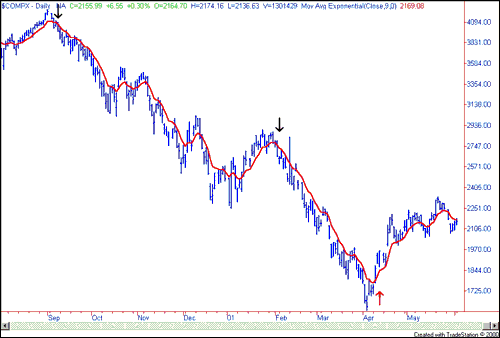
\includegraphics[width=0.8\textwidth]{img/c2/ewa.png}
    \caption{Visualization of exponentially weighted averages.}
    \label{ewa-example}
\end{figure}

\subsubsection{Bias correction in exponentially weighted averages}
The bias correction helps make the exponentially weighted averages more accurate. Because $v(0)=0$, the bias of the weighted averages is shifted and the accuracy suffers at the start.

To solve the bias issue we have to use this equation:

\begin{equation}
    v(t) = \frac{\beta v(t-1) + (1 - \beta) \theta(t)}{(1 - \beta^t)}
\end{equation}

As $t$ becomes larger, $1 - \beta^t$ becomes close to $1$.

\subsubsection{Gradient Descent With Momentum}
The momentum algorithm almost always works faster than standard gradient descent.

The simple idea is to calculate the exponentially weighted average for your gradients and then update your weights with the new values.

Here is the pseudo code:

\begin{lstlisting}[language=python]
vdW = 0, vdb = 0
on iteration t:
    # can be mini-batch or batch gradient descent
    # to compute dW, db on current batch
    
    vdW = beta * vdW + (1 - beta) * dW
    vdb = beta * vdb + (1 - beta) * db
    W = W - learning_rate * vdW
    b = b - learning_rate * vdb
\end{lstlisting}

Momentum helps the cost function to go to the minimum point in a more fast and consistent way.

$\beta$ is a hyperparameter . $\beta = 0.9$ is very common and works very well in most cases. In practice, people don't bother implementing bias correction.

\subsubsection{RMSprop (Root Mean Square prop)}
Here is the pseudo code:
\begin{lstlisting}[language=python]
sdW = 0, sdb = 0
sdW = 0, sdb = 0
on iteration t:
    # can be mini-batch or batch gradient descent
    # compute dw, db on current mini-batch
    
    sdW = (beta * sdW) + (1 - beta) * dW^2  # squaring is element-wise
    sdb = (beta * sdb) + (1 - beta) * db^2  # squaring is element-wise
    W = W - learning_rate * dW / sqrt(sdW)
    b = B - learning_rate * db / sqrt(sdb)
\end{lstlisting}

RMSprop will make the cost function move slower on the vertical direction and faster on the horizontal direction in the following example (Fig. \ref{rmsprop}):

\begin{figure}[!htbp]
    \centering
    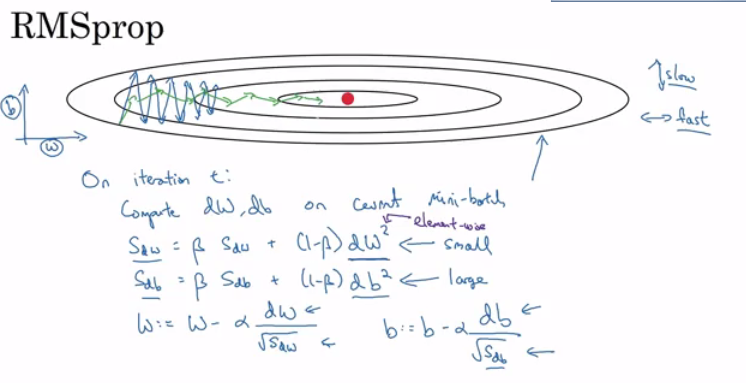
\includegraphics[width=1.0\textwidth, trim={0 0 0 33}, clip]{img/c2/RMSprop.png}
    \caption{Intuition of RMSprop.}
    \label{rmsprop}
\end{figure}

Ensure that $sdW$ is not zero by adding a small value $\epsilon$ (e.g. $\epsilon=10^{-8}$) to it ($\alpha$ represents the learning rate):

\begin{equation}
    W = W - \alpha * \frac{dW}{\sqrt{sdW + \epsilon}}
\end{equation}

With RMSprop you can increase your learning rate. Its developed by Geoffrey Hinton and firstly introduced on Coursera.org course (Neural Networks and Machine Learning).

\subsubsection{Adam Optimization Algorithm}
Stands for Adaptive Moment Estimation.

Adam optimization and RMSprop are among the optimization algorithms that worked very well with a lot of NN architectures.

Adam optimization simply puts RMSprop and momentum together.

Here is the pseudo code:

\begin{lstlisting}[language=python]
vdW = 0, vdW = 0
sdW = 0, sdb = 0
on iteration t:
	# can be mini-batch or batch gradient descent
	# to compute dw, db on current mini-batch                
			
	vdW = (beta1 * vdW) + (1 - beta1) * dW     # momentum
	vdb = (beta1 * vdb) + (1 - beta1) * db     # momentum
			
	sdW = (beta2 * sdW) + (1 - beta2) * dW^2   # RMSprop
	sdb = (beta2 * sdb) + (1 - beta2) * db^2   # RMSprop
			
	vdW = vdW / (1 - beta1^t)      # fixing bias
	vdb = vdb / (1 - beta1^t)      # fixing bias
			
	sdW = sdW / (1 - beta2^t)      # fixing bias
	sdb = sdb / (1 - beta2^t)      # fixing bias
					
	W = W - learning_rate * vdW / (sqrt(sdW) + epsilon)
	b = b - learning_rate * vdb / (sqrt(sdb) + epsilon)
\end{lstlisting}

Here is the equation form:

\begin{equation}
\centering
\begin{aligned}
    vdW &= (\beta_1 * vdW) + (1 - \beta_1) * dW\\
    vdb &= (\beta_1 * vdb) + (1 - \beta_1) * db\\
    sdW &= (\beta_2 * sdW) + (1 - \beta_2) * dW^2\\
    sdb &= (\beta_2 * sdb) + (1 - \beta_2) * db^2\\
    vdW &= vdW / (1 - \beta_1^t)\\
    vdb &= vdb / (1 - \beta_1^t)\\
    sdW &= sdW / (1 - \beta_2^t)\\
    sdb &= sdb / (1 - \beta_2^t)\\
    W &= W - \alpha * \frac{vdW}{\sqrt(sdW) + \epsilon}\\
    b &= b - \alpha * \frac{vdb}{\sqrt(sdW) + \epsilon}
\end{aligned}
\end{equation}

Hyperparameters for Adam:
\begin{itemize}
    \item Learning rate: needed to be tuned.
    \item $\beta_1$: parameter of the momentum - 0.9 is recommended by default.
    \item $\beta_2$: parameter of the RMSprop - 0.999 is recommended by default.
    \item $\epsilon$: $10^-8$ is recommended by default.
\end{itemize}

\subsubsection{Learning Rate Decay}
Slowly reduce learning rate.

As mentioned before mini-batch gradient descent won't reach the optimum point (converge). But by making the learning rate decay with iterations it will be much closer to it because the steps (and possible oscillations) near the optimum are smaller.

% One technique equation is \textit{learning\_rate = (1 / (1 + decay\_rate * epoch\_num)) * learning\_rate\_0}.

Several popular decay rate decay ($r$ represents the decay rate and i represents the current number of epoch):

\begin{equation}
    \begin{aligned}
        \alpha &= \frac{1}{1 + r * i} * \alpha_0\\
        \alpha &= 0.95^i * \alpha_0\\
        \alpha &= \frac{k}{\sqrt{i}} * \alpha_0
    \end{aligned}
\end{equation}

Besides, some people perform learning rate decay discretely - repeatedly decrease after some number of epochs. While also some people are making changes to the learning rate manually.

decay\_rate $r$  is another hyperparameter which has less priority.

\subsubsection{The Problem of Local Optima}
The normal local optima is not likely to appear in a deep neural network because data is usually high dimensional. For point to be a local optima it has to be a local optima for each of the dimensions which is highly unlikely.

It's unlikely to get stuck in a bad local optima in high dimensions, it is much more likely to get to the saddle point rather to the local optima, which is not a problem.

Plateaus can make learning slow:
\begin{itemize}
    \item Plateau is a region where the derivative is close to zero for a long time.
    \item This is where algorithms like momentum, RMSprop or Adam can help.
\end{itemize}

\subsection{Hyperparameter Tuning, Batch Normalization and Programming Frameworks}
\subsubsection{Tuning Process}
We need to tune our hyperparameters to get the best out of them.

Hyperparameters importance are (as for Andrew Ng, importance doesn't decrease strictly):

\begin{itemize}
    \item[i.] Learning rate
    \item[ii.] Momentum beta
    \item[iii.] Mini-batch size
    \item[iv.] No. of hidden units
    \item[v.] No. of layers
    \item[vi.] Learning rate decay
    \item[vii.] Regularization lambda
    \item[viii.] Activation functions
    \item[ix.] Adam $\beta_1$, $\beta_2$ and $\epsilon$
\end{itemize}

It's hard to decide which hyperparameter is the most important in a problem. It depends a lot on your problem.

One of the ways to tune is to sample a grid with N hyperparameters settings and then try all settings combinations on your problem.

However, try random values instead of using a grid.

You can use Coarse to fine sampling scheme:

\begin{itemize}
    \item When you find some hyperparameters values that give you a better performance - zoom into a smaller region around these values and sample more densely within this space.
\end{itemize}

\subsubsection{Using an Appropriate Scale to Pick Hyperparameters}
Let's say you have a specific range for a hyperparameter from $a$ to $b$. It's better to search for the right ones using the logarithmic scale rather than in linear scale:

\begin{itemize}
    \item Calculate: a\_log = log(a), e.g. a = 0.0001 then a\_log = -4
    \item Calculate: b\_log = log(b), e.g. b = 1 then b\_log = 0
    \item Then: r = (a\_log - b\_log), result = 10\^r
\end{itemize}

It uniformly samples values in log scale from [a, b].

If you want to use the last method on exploring on the "momentum beta $\beta$":

i. $\beta$ best range is from 0.9 to 0.999.

ii. You should search for $1-\beta$ in range 0.001 to 0.1 and then replace a with 0.001 and replace b with 0.1.

\subsubsection{Hyperparameters Tuning in Practice: Pandas vs. Caviar}
Intuitions about hyperparameter settings from one application area may or may not transfer to a different one.

If you don't have much computational resources you can use "babysitting model":
\begin{itemize}
    \item Day 0 you might initialize your parameter as random and then start training.
    \item Then you watch your learning curve gradually decrease over the day.
    \item And each day you nudge your parameters a little during training.
    \item Called panda approach.
\end{itemize}

If you have enough computational resources, you can run some models in parallel and at the end of the day(s) you check the results.

\begin{itemize}
    \item Called Caviar approach.
\end{itemize}

\subsubsection{Normalizing Activations in a Network}

Batch Normalization can speed up learning.

Before we normalized input by subtracting the mean and dividing by variance. This helped a lot for the shape of the cost function and for reaching the minimum point faster.

The question is: for any hidden layer can we normalize A[l] to train W[l+1], b[l+1] faster? This is what batch normalization is about.

There are some debates in the deep learning literature about whether you should normalize values before the activation function Z[l] or after applying the activation function A[l]. In practice, normalizing Z[l] is done much more often and that is what Andrew Ng presents.

% https://github.com/mbadry1/DeepLearning.ai-Summary/tree/master/2-%20Improving%20Deep%20Neural%20Networks#normalizing-activations-in-a-network

Algorithm:

\begin{lstlisting}
1. Given Z[l] = [z(1), ..., z(m)], i = 1 to m (for each input)
2. Compute mean = 1/m * sum(z(i))
3. Compute variance = 1/m * sum(z(i) - mean)^2
4. Then Z_norm[l] = (z[l] - mean) / np.sqrt(variance + epsilon) 
    Forcing the inputs to a distribution with zero mean and 1 variance
5. Then Z_tilde[l] = gamma * Z_norm[l] + beta 
    To make inputs belong to other distribution; 
    Gamma and beta are learnable parameters of the model; 
    Making the NN learn the distribution of the outputs.
\end{lstlisting}

\subsubsection{Fitting Batch Normalization into a Neural Network}
Using batch norm in 2 layers NN:

\begin{figure}[!hbtp]
    \centering
    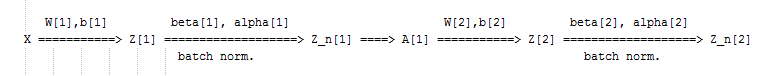
\includegraphics[width=1.0\textwidth]{img/c2/bn.png}
    \caption{Workflow of 2 layers NN with batch normalization.}
    \label{fig:my_label}
\end{figure}

$\beta[i]$ and $\gamma[i]$ are updated using any optimization algorithms (like GD, Momentum, RMSprop, Adam).

Batch normalization is usually applied with mini-batches.

Shapes: $Z[l] - (n[l], m), \beta[l] - (n[l], m), \gamma[l] - (n[l], m)$.

\subsubsection{Why Does Batch Normalization Work?}
The first reason is the same reason as why we normalize X (Shape the inputs and makes loss reach minimum point faster).

The second reason is that batch normalization reduces the problem of input values changing (shifting).

\subsubsection{Batch Normalization at Test Time}
When we train a NN with batch normalization, we compute the mean and the variance of the mini-batch.

In testing we might need to process examples one at a time. The mean and the variance of one example won't make sense. We have to compute an estimated value of mean and variance to use it in testing time.

We can use the weighted average cross the mini-batches. We will use the estimated values of the mean and variance to test. This method is also sometimes called "running average".

In practice most often you will use a deep learning framework and it will contain some default implementation of doing such a thing.

\subsubsection{Softmax Regression}
In every example we have used so far we were talking about binary classification. There are a generalization of logistic regression called softmax regression that is used for multiclass classification/regression.

Each of C values in the output layer will contain a probability of the example to belong to each of the classes. In the last layer we will have to activate the softmax activation function instead of the sigmoid activation.

\begin{equation}
    A[L] = \frac{e^{z[L]}}{\sum e^{z[L]}}
\end{equation}

\subsubsection{Training a Softmax Classifier}
There is an activation which is called hard max, which gets 1 for the maximum value and zeros for the others. If you are using NumPy, it's np.max over the vertical axis.

The softmax name came from softening the values and not harding them like hard max.

Softmax is a generalization of logistic activation function to C classes. If C = 2 softmax reduces to logistic regression.

The loss function used with softmax:

\begin{equation}
    L (y, \hat{y}) = - \sum y_j * \log \hat{y}_j,\ \ j: 0\to C-1
\end{equation}

With m examples:

\begin{equation}
    L (Y, \hat{Y}) = - \frac{1}{m} \sum y_j^{(i)} * \log \hat{y}_j^{(i)},\ \ j: 0\to C-1, i: 0\to m
\end{equation}

Back propagation with softmax:

\begin{equation}
    dZ[L] = \hat{Y} - Y
\end{equation}

That's all for Course II: Improving Deep Neural Networks: Hyperparameter tuning, Regularization and Optimization.

\newpage

